
%------------------------------------------
\subsubsection{Linear basis functions ($Q_1$)}
\index{$Q_1$}

Let $f(r)$ be a $C^1$ function on the interval $[-1:1]$ with $f(-1)=f_1$  and $f(1)=f_2$.
\begin{center}
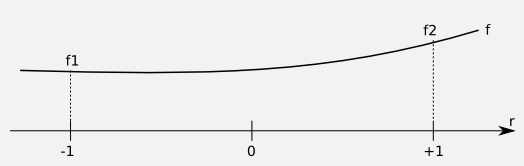
\includegraphics[width=8cm]{images/linshapefct.png}
\end{center}
Let us assume that the function $f(r)$ is to be approximated on $[-1,1]$ by the first order polynomial 
\begin{equation}
f(r)=a+br \label{eqquad1}
\end{equation}
Then it must fulfill
\begin{eqnarray}
f(r=-1)&=&a-b =f_1 \nonumber\\
f(r=+1)&=&a+b =f_2 \nonumber
\end{eqnarray}
This leads to  
\[
a=\frac{1}{2}(f_1+f_2)  
\quad\quad
b=\frac{1}{2}(-f_1+f_2)  
\]
and then replacing $a,b$ in Eq. (\ref{eqquad1}) by the above values on gets
\[
f(r) = \left[  \frac{1}{2}(1-r)\right] f_1 + \left[ \frac{1}{2}(1+r) \right] f_2
\]
or
\[
f(r)=\sum_{i=1}^2 N_i(r) f_1
\]
with
\begin{mdframed}[backgroundcolor=blue!5]
\begin{eqnarray}
N_1(r) &=& \frac{1}{2} (1-r) \nonumber\\
N_2(r) &=& \frac{1}{2} (1+r)
\end{eqnarray}
\end{mdframed}

\begin{center}
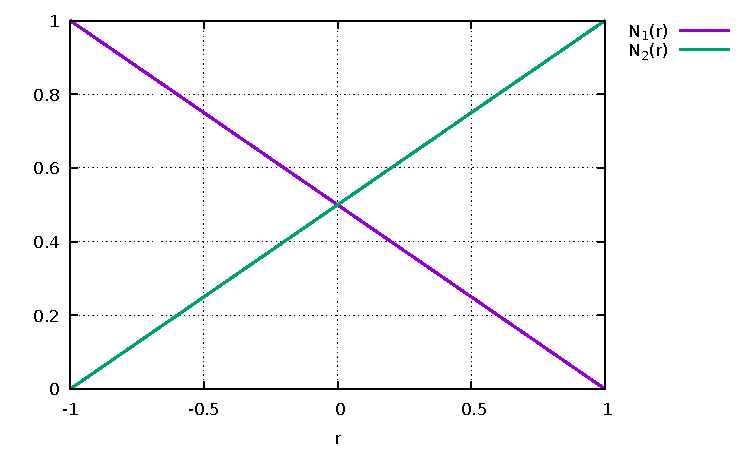
\includegraphics[width=6cm]{images/basis1D/linear.pdf}
\end{center}

%------------------------------------------
\subsubsection{Quadratic basis functions ($Q_2$)}
\index{$Q_2$}

Let $f(r)$ be a $C^1$ function on the interval $[-1:1]$ with $f(-1)=f_1$, $f(0)=f_2$ and $f(1)=f_3$.
\begin{center}
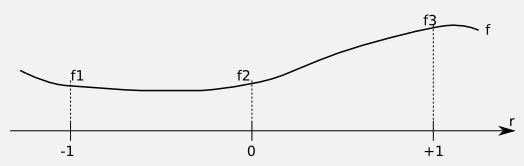
\includegraphics[width=8cm]{images/quadshapefct.png}
\end{center}

Let us assume that the function $f(r)$ is to be approximated on $[-1,1]$ by the second order polynomial
\begin{equation}
f(r)=a+br+cr^2 \label{eqquad}
\end{equation}
Then it must fulfill
\begin{eqnarray}
f(r=-1)&=&a-b+c = f_1 \nonumber\\
f(r=0) &=&a\quad\quad\quad\;     = f_2 \nonumber\\
f(r=+1)&=&a+b+c = f_3 \nonumber
\end{eqnarray}
This leads to
\[
a=f_2 
\quad
b=\frac{1}{2}(-f1+f3)
\quad
c=\frac{1}{2}(f_1+f_3-2f_2)
\]
and then replacing $a,b,c$ in Eq. (\ref{eqquad}) by the above values on gets
\[
f(r)=\left[\frac{1}{2}r(r-1)\right] f_1 + (1-r^2) f_2 + \left[\frac{1}{2}r(r+1)\right] f_3
\]
or,
\[
f(r) = \sum_{i=1}^3 N_i(r) f_i
\]
with
\begin{mdframed}[backgroundcolor=blue!5]
\begin{eqnarray}
N_1(r) &=& \frac{1}{2}r(r-1) \nonumber\\
N_2(r) &=& (1-r^2) \nonumber\\ 
N_3(r) &=& \frac{1}{2}r(r+1) 
\end{eqnarray}
\end{mdframed}

\begin{center}
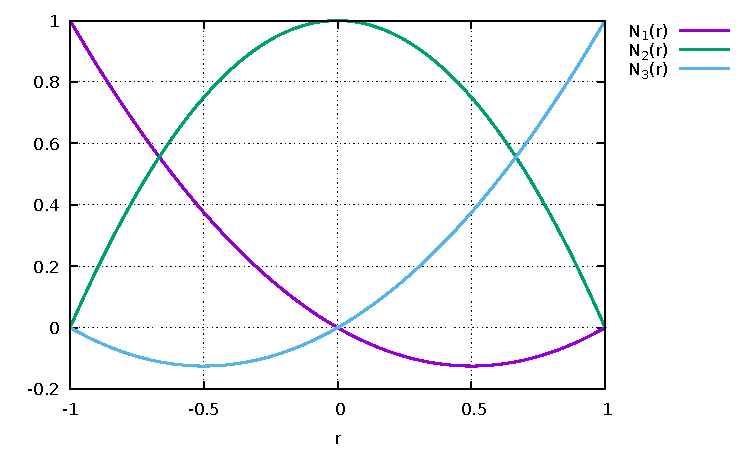
\includegraphics[width=6cm]{images/basis1D/quadratic.pdf}
\end{center}


%------------------------------------------
\subsubsection{Cubic basis functions ($Q_3$)}
\index{$Q_3$}

The 1D basis polynomial is given by
\[
f(r)=a+br+cr^2+dr^3
\]
with the nodes at position -1,-1/3, +1/3 and +1.

\begin{eqnarray}
f(-1)   &=& a-b+c-d = f_1 \nonumber\\
f(-1/3) &=& a-\frac{b}{3}+\frac{c}{9}-\frac{d}{27} = f_2 \nonumber\\
f(+1/3) &=& a-\frac{b}{3}+\frac{c}{9}-\frac{d}{27} = f_3 \nonumber\\
f(+1)   &=& a+b+c+d = f_4 \nonumber
\end{eqnarray}

Adding the first and fourth equation and the second and third, one arrives at
\[
f_1+f_4 = 2a+2c \quad\quad\quad f_2+f_3=2a+\frac{2c}{9}
\]
and finally:
\[
a=\frac{1}{16} \left( -f_1 + 9f_2 + 9f_3 - f_4  \right)
\]
\[
c=\frac{9}{16}\left(f_1-f_2-f_3+f_4\right)
\]
Combining the original 4 equations in a different way yields
\[
2b+2d=f_4-f_1 
\quad\quad\quad
\frac{2b}{3} + \frac{2d}{27} = f_3-f_2
\]
so that
\[
b=\frac{1}{16} \left( f_1 - 27f_2 + 27f_3 -f_4   \right)
\]
\[
d=\frac{9}{16} \left( -f_1 + 3f_2 - 3f_3 + f_4 \right)
\]
Finally,

\begin{eqnarray}
f(r) 
&=& a+b+cr^2+dr^3 \nonumber\\
&=& \frac{1}{16} (-1+  r +9r^2 - 9r^3 )f_1 \nonumber\\ 
&+& \frac{1}{16} ( 9-27r -9r^2 +27r^3 )f_2 \nonumber\\ 
&+& \frac{1}{16} ( 9+27r -9r^2 -27r^3 )f_3 \nonumber\\ 
&+& \frac{1}{16} (-1-  r +9r^2 + 9r^3 )f_4 \nonumber\\ 
&=& \sum_{i=1}^4 N_i(r) f_i \nonumber
\end{eqnarray}
where
\begin{mdframed}[backgroundcolor=blue!5]
\begin{eqnarray}
N_1&=& \frac{1}{16} (-1+  r+9r^2- 9r^3 ) \nonumber\\ 
N_2&=& \frac{1}{16} ( 9-27r-9r^2+27r^3 ) \nonumber\\ 
N_3&=& \frac{1}{16} ( 9+27r-9r^2-27r^3 ) \nonumber\\ 
N_4&=& \frac{1}{16} (-1-  r+9r^2+ 9r^3 ) \nonumber
\end{eqnarray}
\end{mdframed}

\begin{center}
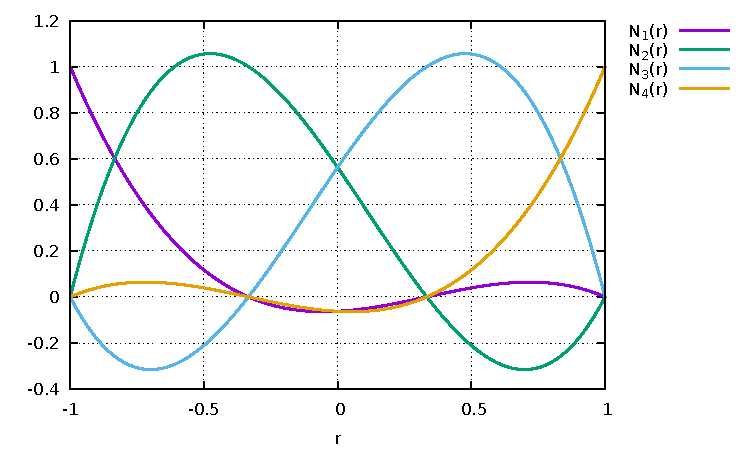
\includegraphics[width=6cm]{images/basis1D/cubic.pdf}
\end{center}


Verification:

\begin{itemize}
\item
Let us assume $f(r)=C$, then
\[
\hat{f}(r) = \sum N_i(r) f_i = \sum_i N_i C = C \sum_i N_i  = C
\]
so that a constant function is exactly reproduced, as expected.

\item
Let us assume $f(r)= r$, then $f_1=-1$, $f_2=-1/3$, $f_3=1/3$ and $f_4=+1$. We then have
\begin{eqnarray}
\hat{f}(r) 
&=& \sum N_i(r) f_i  \nonumber\\
&=& - N_1(r) -\frac{1}{3}N_2(r) + \frac{1}{3}N_3(r)  + N_4(r) \nonumber\\
&=& [-(-1+  r+9r^2- 9r^3 ) \nn\\
&&- \frac{1}{3} ( 9-27r-9r^2-27r^3 ) \nn\\
&&+ \frac{1}{3} ( 9+27r-9r^2+27r^3 ) \nn\\
&&+ (-1-  r+9r^2+ 9r^3 )]/16 \nonumber\\
&=& [-r +9r + 9r -r]/16  + ... 0 ... \nonumber\\
&=& r   
\end{eqnarray}

\end{itemize}


The basis functions derivative are given by
\begin{mdframed}[backgroundcolor=blue!5]
\begin{eqnarray}
 \frac{\partial N_1}{\partial r}&=& \frac{1}{16}  (  1 +18r - 27r^2 ) \nonumber\\ 
 \frac{\partial N_2}{\partial r}&=& \frac{1}{16}  (-27 -18r + 81r^2 ) \nonumber\\ 
 \frac{\partial N_3}{\partial r}&=& \frac{1}{16}  (+27 -18r - 81r^2 ) \nonumber\\ 
 \frac{\partial N_4}{\partial r}&=& \frac{1}{16}  ( -1 +18r + 27r^2 ) \nonumber
\end{eqnarray}
\end{mdframed}
Verification:

\begin{itemize}
\item
Let us assume $f(r)=C$, then
\begin{eqnarray}
\frac{\partial \hat{f}}{\partial r} 
&=& \sum_i \frac{\partial N_i}{\partial r} f_i  \nonumber\\
&=&  C \sum_i \frac{\partial N_i}{\partial r}  \nonumber\\
&=& \frac{C}{16} [  (  1 +18r - 27r^2 ) \nn\\
&&+ (-27 -18r + 81r^2 )  \nn\\
&&+  (+27 -18r - 81r^2 ) \nn\\
&&+ ( -1 +18r + 27r^2 ) ]  \nonumber\\
&=& 0 \nonumber
\end{eqnarray}

\item
Let us assume $f(r)= r$, then $f_1=-1$, $f_2=-1/3$, $f_3=1/3$ and $f_4=+1$. We then have
\begin{eqnarray}
\frac{\partial \hat{f}}{\partial r} 
&=& \sum_i \frac{\partial N_i}{\partial r} f_i  \nonumber\\
&=& \frac{1}{16} [  -(  1 +18r - 27r^2 ) \nn\\ 
&& -\frac{1}{3} (-27 -18r + 81r^2 )  \nn\\
&& +\frac{1}{3}  (+27 -18r - 81r^2 ) \nn\\
&& + ( -1 +18r + 27r^2 ) ]  \nonumber\\
&=& \frac{1}{16} [-2 + 18 + 54r^2 - 54r^2] \nonumber\\
&=& 1 \nonumber
\end{eqnarray}

\end{itemize}

%------------------------------------------
\subsubsection{Quartic basis functions ($Q_4$)}
\index{$Q_4$}

The 1D basis polynomial is given by
\[
f(r)=a+br+cr^2+dr^3+er^4
\]
with the nodes at position -1,-1/2, 0, +1/2 and +1.

\begin{eqnarray}
f(-1)   &=& a-b+c-d+e = f_1 \nonumber\\
f(-1/2) &=& a-\frac{b}{2}+\frac{c}{4}-\frac{d}{8}+\frac{e}{16} = f_2 \nonumber\\
f(0)    &=& a = f_3 \nonumber\\
f(+1/2) &=& a-\frac{b}{2}+\frac{c}{4}-\frac{d}{8}+\frac{e}{16} = f_4 \nonumber\\
f(+1)   &=& a+b+c+d+e = f_5 \nonumber
\end{eqnarray}
or, 
\begin{equation}
\left(
\begin{array}{ccccc}
 1  &  -1  &  1 &  -1 &  1 \\ 
 1  &  -1/2  &  1/4 &  -1/8 &  1/16 \\ 
 1  &   0    &  0   &   0   & 0 \\
 1  &  1/2  &  1/4 &  1/8 &  1/16 \\ 
 1  &  1  &  1 &  1 &  1 
\end{array}
\right)
\left(
\begin{array}{c}
a \\ b \\ c \\ d \\ e
\end{array}
\right)
=
\left(
\begin{array}{c}
f_1 \\ f_2 \\ f_3 \\ f_4 \\ f_5
\end{array}
\right)
\end{equation}

The third line gives $a=f_3$ so that
\begin{equation}
\underbrace{
\left(
\begin{array}{ccccc}
-1  &  1   &  -1 &  1 \\ 
-1/2 &  1/4 & -1/8 &  1/16 \\ 
 1/2 &  1/4 &  1/8 &  1/16 \\ 
 1  &  1   &  1 &  1 
\end{array}
\right)}_{A}
\left(
\begin{array}{c}
b \\ c  \\ d \\ e
\end{array}
\right)
=
\left(
\begin{array}{c}
f_1 -f_3 \\ f_2 -f_3\\ f_4-f_3 \\ f_5 -f_3
\end{array}
\right)
\end{equation}
The inverse of the matrix $A$ is:
\[
A^{-1}=
\frac{1}{6}
\left(
\begin{array}{ccccc}
1 & -8 & 8 & -1 \\
-1 & 16 & 16 & -1 \\
-4 & 8 & -8 & 4 \\
4 & -16 & -16 & 4
\end{array}
\right)
\]
so that 
\[
\left(
\begin{array}{c}
b \\ c \\ d \\ e
\end{array}
\right)
=
\frac{1}{6}
\left(
\begin{array}{ccccc}
1 & -8 & 8 & -1 \\
-1 & 16 & 16 & -1 \\
-4 & 8 & -8 & 4 \\
4 & -16 & -16 & 4
\end{array}
\right)
\cdot
\left(
\begin{array}{c}
f_1 -f_3 \\ f_2 -f_3\\ f_4-f_3 \\ f_5 -f_3
\end{array}
\right)
\]

and then 
\begin{eqnarray}
b &=& \frac{1}{6} \left( f_1 -8f_2 +8 f_4 -f_5     \right) \\
c &=& \frac{1}{6} \left( -f_1 +16f_2 -30f_3    + 16f_4- f_5   \right) \\
d &=& \frac{1}{6} \left( -4f_1 +8f_2     -8f_4+ 4 f_5   \right) \\
e &=& \frac{1}{6} \left( 4f_1 -16f_2 +24f_3 -16f_4+ 4 f_5   \right) 
\end{eqnarray}

\begin{eqnarray}
f(r) 
&=& a+br+cr^2+dr^3+er^4 \\
&=& f_3 + 
\frac{1}{6} \left( f_1 -8f_2 +8 f_4 -f_5     \right)  r  +
\frac{1}{6} \left( -f_1 +16f_2 -30f_3    + 16f_4- f_5   \right) r^2 +\\ &&
\frac{1}{6} \left( -4f_1 +8f_2     -8f_4+ 4 f_5   \right) r^3 +
\frac{1}{6} \left( 4f_1 -16f_2 +24f_3 -16f_4+ 4 f_5   \right) r^4 \\
&=& \frac{1}{6} \left(  r- r^2 -4r^3 +4r^4\right) f_1 \\
&+& \frac{1}{6} \left(  -8r+16 r^2 +8r^3 -16 r^4\right) f_2 \\
&+& \left( 1 -5r^2+4r^4  \right) f_3 \\
&+& \frac{1}{6} \left(  8r+16 r^2 -8r^3 -16 r^4\right) f_4 \\
&+& \frac{1}{6} \left(  -r- r^2 +4r^3 +4r^4\right) f_5
\end{eqnarray}

Finally
\begin{mdframed}[backgroundcolor=blue!5]
\begin{eqnarray}
N_1(r)&=& \frac{1}{6} \left(  r- r^2 -4r^3 +4r^4\right) \\
N_2(r)&=& \frac{1}{6} \left(  -8r+16 r^2 +8r^3 -16 r^4\right)  \\
N_3(r)&=& \left( 1 -5r^2+4r^4  \right)  \\
N_4(r)&=& \frac{1}{6} \left(  8r+16 r^2 -8r^3 -16 r^4\right)  \\
N_5(r)&=& \frac{1}{6} \left(  -r- r^2 +4r^3 +4r^4\right) 
\end{eqnarray}
\end{mdframed}


\begin{center}
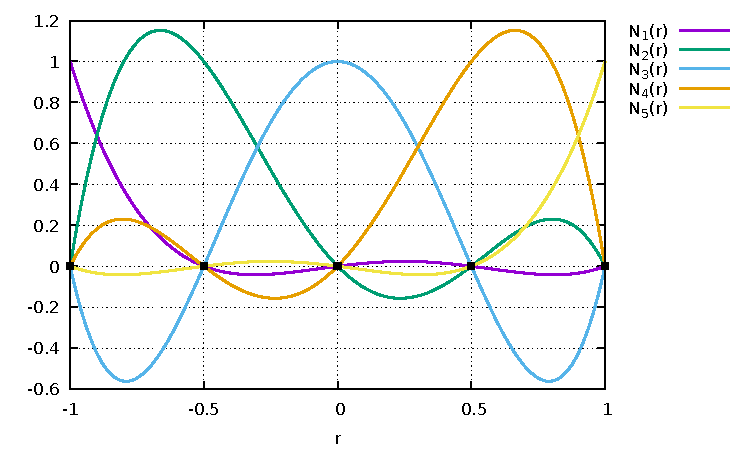
\includegraphics[width=6cm]{images/basis1D/quartic.pdf}
\end{center}




